% +------------------------------------------------------------------------+
% | Reference manual page: Periodic_3_triangulation_3.tex
% +------------------------------------------------------------------------+
% | 19.2.2009   Monique Teillaud, Manuel Caroli
% | Package: Periodic_3_triangulation_3
% | 
\RCSdef{\RCSPeriodictriangulationRev}{$Id$}
\RCSdefDate{\RCSPeriodictriangulationDate}{$Date$}
% |
%%RefPage: end of header, begin of main body
% +------------------------------------------------------------------------+


\begin{ccRefClass}{Periodic_3_triangulation_3<PT,TDS>}

\ccDefinition

The class \ccc{Periodic_triangulation_3} represents a 3-dimensional
triangulation of a point set in $\mathbb T_c^3$.

\ccInclude{CGAL/Periodic_3_triangulation_3.h}

\ccParameters

The first template argument \ccc{PT} must be a model of the
\ccc{Periodic_3DelaunayTriangulationTraits_3} concept.

The second template argument \ccc{TDS} must be a model of the
\ccc{TriangulationDataStructure_3} concept with some additional
functionality in cells and vertices.
Its default value is
\ccc{Triangulation_data_structure_3<Triangulation_vertex_base_3<PT,Periodic_3_triangulation_ds_vertex_base_3<>>,Triangulation_cell_base_3<PT,Periodic_3_triangulation_ds_cell_base_3<>>>}. 

\ccTypes
The class \ccc{Triangulation_3} defines the following types:
\ccThree{typedef Geometric_traits::Periodic_3_offset_3}{Covering_sheets;}{}
\ccThreeToTwo

\ccTypedef{typedef PT Geometric_traits;}{}
\ccGlue
\ccTypedef{typedef TDS Triangulation_data_structure;}{}

\ccTypedef{typedef Geometric_traits::Periodic_3_offset_3
  Offset;}{}
\ccGlue
\ccTypedef{typedef Geometric_traits::Iso_cuboid_3 Iso_cuboid;} 
{A type representing an axis-aligned cuboid. It must be a model of \ccc{PT::Iso_cuboid_3}. Used to represent the original domain.}
\ccGlue
\ccTypedef{typedef array<int,3> Covering_sheets;}{Integer triple to
  store the number of sheets in each direction of space.}

\ccTypedef{typedef Geometric_traits::Point_3 Point;}{}
\ccGlue
\ccTypedef{typedef Geometric_traits::Segment_3 Segment;}{}
\ccGlue
\ccTypedef{typedef Geometric_traits::Triangle_3 Triangle;}{}
\ccGlue
\ccTypedef{typedef Geometric_traits::Tetrahedron_3 Tetrahedron;}{}

\ccTypedef{typedef std::pair< Point, Offset >
  Periodic_point;}{}
\ccGlue
\ccTypedef{typedef array< Periodic_point, 2>
  Periodic_segment;}{}
\ccGlue
\ccTypedef{typedef array< Periodic_point, 3>
  Periodic_triangle;}{}
\ccGlue
\ccTypedef{typedef array< Periodic_point, 4>
  Periodic_tetrahedron;}{}

Only vertices ($0$-faces) and cells ($3$-faces) are stored. Edges
($1$-faces) and facets ($2$-faces) are not explicitly represented and
thus there are no corresponding classes (see
Section~\ref{P3Triangulation3-sec-intro}).

\ccTypedef{typedef Triangulation_data_structure::Vertex Vertex;}{}
\ccGlue
\ccTypedef{typedef Triangulation_data_structure::Cell Cell;}{}
\ccGlue
\ccTypedef{typedef Triangulation_data_structure::Edge Edge;}{}
\ccGlue
\ccTypedef{typedef Triangulation_data_structure::Facet Facet;}{}

The vertices and faces of the triangulations are accessed through
\ccc{handles}, \ccc{iterators} and \ccc{circulators}. 
A handle is a type which supports the two dereference operators
\ccc{operator*} and \ccc{operator->}.  The Handle concept is
documented in the support library.
Iterators and circulators are bidirectional and non-mutable.
The edges and facets of the triangulation can also be visited through
iterators and circulators which are bidirectional and non-mutable.

Iterators and circulators are convertible to the corresponding handles, thus
the user can pass them directly as arguments to the functions.

\ccThree{typedef Triangulation_data_structure::Facet_circulator}{Facet_circulator;}{}
\ccThreeToTwo

\ccTypedef{typedef Triangulation_data_structure::Vertex_handle Vertex_handle;}
{handle to a vertex}
\ccGlue
\ccTypedef{typedef Triangulation_data_structure::Cell_handle Cell_handle;}
{handle to a cell}

\ccTypedef{typedef Triangulation_data_structure::size_type size_type;}
{Size type (an unsigned integral type)}
\ccGlue
\ccTypedef{typedef Triangulation_data_structure::difference_type difference_type;}
{Difference type (a signed integral type)}

\ccTypedef{typedef Triangulation_data_structure::Cell_iterator Cell_iterator;}
{iterator over cells}
\ccGlue
\ccTypedef{typedef Triangulation_data_structure::Facet_iterator Facet_iterator;}
{iterator over facets}
\ccGlue
\ccTypedef{typedef Triangulation_data_structure::Edge_iterator Edge_iterator;}
{iterator over edges}
\ccGlue
\ccTypedef{typedef Triangulation_data_structure::Vertex_iterator Vertex_iterator;}
{iterator over vertices}

\ccTypedef{typedef Triangulation_data_structure::Cell_circulator Cell_circulator;}
{circulator over all cells incident to a given edge} 
\ccGlue
\ccTypedef{typedef Triangulation_data_structure::Facet_circulator Facet_circulator;}
{circulator over all facets incident to a given edge}

\ccTwo{Periodic_3_triangulation_3<PT,TDS>:: Periodic_tetrahedron_iterator}{}

\ccHeading{Geometric iterators:}
\ccNestedType{Periodic_tetrahedron_iterator}{iterator over the tetrahedra
  corresponding to cells of the triangulation.}
\ccGlue
\ccNestedType{Periodic_triangle_iterator}{iterator over the triangles
  corresponding to facets of the triangulation.}
\ccGlue
\ccNestedType{Periodic_segment_iterator}{iterator over the segments
  corresponding to edges of the triangulation.}
\ccGlue
\ccNestedType{Periodic_point_iterator}{iterator over the points
  corresponding to vertices of the triangulation.}
\ccGlue

\ccThree{typedef Geometric_traits::Tetrahedron Tetrahedro;}{T}{}
\ccThreeToTwo

\ccHeading{Enums:}
The triangulation class also defines the following enum types:

To specify which case occurs when locating a point in the triangulation.\\
\ccEnum{enum Locate_type {VERTEX=0, EDGE, FACET, CELL, EMPTY};}{}

To specify the behavior of geometric iterators.\\
\ccEnum{enum Iterator_type {STORED=0, UNIQUE, STORED_COVER_DOMAIN,
    UNIQUE_COVER_DOMAIN};}{} 

\ccCreation
\ccCreationVariable{t}  %% choose variable name

\ccThree{Periodic_3_triangulation_3<>}{Facetxxx }{}

\ccConstructor{Periodic_3_triangulation_3
(const Iso_cuboid & domain = Iso_cuboid(0,0,0,1,1,1),
 const Geometric_traits & traits = Geometric_traits());} 
{Introduces an empty triangulation \ccVar\ with \ccc{domain} as
  original domain.
\ccPrecond{\ccc{domain} is a cube.}}

\ccConstructor{Periodic_3_triangulation_3 (const Periodic_3_triangulation_3 & tr);} 
{Copy constructor. All vertices and faces are duplicated.}

\ccHeading{Assignment}

\ccThree{Periodic_3_triangualtion_3 &}{t.clear()x}{}

\ccMethod{Periodic_3_triangulation_3 & operator=(const Periodic_3_triangulation_3 & tr);}
{The triangulation \ccc{tr} is duplicated, and modifying the copy after the 
duplication does not modify the original. The previous triangulation held
by \ccVar\ is deleted.}

\ccMethod{void swap(Periodic_3_triangulation_3 & tr);}
{The triangulations \ccc{tr} and \ccVar\ are swapped.
\ccVar.\ccc{swap(tr)} should be preferred to \ccVar\ = \ccc{tr} or to
\ccc{t(tr)} if \ccc{tr} is deleted after that. Indeed, there is no
copy of cells and vertices, thus this method runs in constant time.}

\ccMethod{void clear();}
{Deletes all vertices and all cells of \ccVar.}

\ccFunction{template < class PT, class TDS1, class TDS2 >
            bool operator==(const Periodic_3_triangulation_3<PT, TDS1> & t1,
                            const Periodic_3_triangulation_3<PT, TDS2> & t2);}
{Equality operator.  Returns true iff there exist a bijection between the
vertices of \ccc{t1} and those of \ccc{t2} and a bijection between the cells of
\ccc{t1} and those of \ccc{t2}, which preserve the geometry of the
triangulation, that is, the points of each corresponding pair of vertices are
equal, and the tetrahedra corresponding to each pair of cells are equal (up to
a permutation of their vertices).}
\ccGlue
\ccFunction{template < class PT, class TDS1, class TDS2 >
            bool operator!=(const Periodic_3_triangulation_3<PT, TDS1> & t1,
                            const Periodic_3_triangulation_3<PT, TDS2> & t2);}
{The opposite of \ccc{operator==}.}

\ccAccessFunctions

\ccThree{Triangulation_data_structure &}{t.number_of_sheets()x}{}

\ccMethod{const Geometric_traits & geom_traits() const;}
{Returns a const reference to the geometric traits object.}
\ccGlue
\ccMethod{const Triangulation_data_structure & tds() const;}
{Returns a const reference to the triangulation data structure.}

\begin{ccAdvanced}
\ccHeading{Non const access}
The responsibility of keeping a valid triangulation belongs to the user
when using advanced operations allowing a direct manipulation of the \ccc{tds}.
This method is mainly a help for users implementing their own triangulation
algorithms.

\ccMethod{Triangulation_data_structure & tds();}
{Returns a reference to the triangulation data structure.}
\end{ccAdvanced}

\ccMethod{Iso_cuboid domain() const;}
{Returns the original domain.}

\begin{ccAdvanced}
\ccMethod{Covering_sheets number_of_sheets() const;}
{Returns the number of sheets of the covering the triangulation is
  currently computed in.} 

\ccThree{bool}{t.is_extensible_triangulation_in_1_sheet_h2()x}{}
\ccHeading{Non-constant-time queries and conversions}
\ccMethod{bool is_extensible_triangulation_in_1_sheet_h1() const;}
{The current triangulation remains a triangulation in 1-sheeted
  covering even after adding points if this method returns
  \ccc{true}. This test relies on a heuristic, i.e.\ if it answers
  \ccc{false} nothing is known. This test runs in constant-time when
  not computing in 1-sheeted covering space. (This test uses the length
of the longest edge in the triangulation as a
criterion \cite{cgal:ct-c3dpt-09}.)}

\ccMethod{bool is_extensible_triangulation_in_1_sheet_h2() const;}
{The same as \ccc{is_extensible_triangulation_in_1_sheet_h1()} but with
a more precise heuristic, i.e.\ it might answer \ccc{true} in cases in which
\ccc{is_extensible_triangulation_in_1_sheet_h1()} would not. However, it is
much less time efficient when not computing in 1-sheeted covering
space. (This test uses the diameter of the largest empty ball in the
input point set as a criterion \cite{cgal:ct-c3dpt-09}.)}
\ccGlue
\ccMethod{bool is_triangulation_in_1_sheet() const;}
{Returns \ccc{true} if the current triangulation would still be a
  triangulation in 1-sheeted covering, returns \ccc{false} otherwise.}

It is not recommended to interfere with the built-in covering
management. Especially a premature conversion to a 1-sheeted covering
might lead to problems when modifying the triangulation later.
\ccMethod{void convert_to_1_sheeted_covering() const;}
{Converts the current triangulation into the same periodic
  triangulation in 1-sheeted covering.}
\ccGlue
\ccMethod{void convert_to_27_sheeted_covering() const;}
{Converts the current triangulation into the same periodic
  triangulation in 27-sheeted covering.}

\end{ccAdvanced}

\ccThree{size_type}{t.number_of_stored_vertices()}{}

\ccMethod{size_type number_of_vertices() const;}
{Returns the number of vertices. Counts all vertices that are
  representatives of the same point in $\mathbb T_c^3$ as one vertex.}
\ccGlue
\ccMethod{size_type number_of_cells() const;}
{Returns the number of cells. Counts all cells that are
  representatives of the same tetrahedron in $\mathbb T_c^3$ as one
  cell.}

\begin{ccAdvanced}
\ccMethod{size_type number_of_stored_vertices() const;}
{Returns the number of vertices in the data structure. This is the
  same as the number of sheets times \ccc{number_of_vertices()}. }
\ccGlue
\ccMethod{size_type number_of_stored_cells() const;}
{Returns the number of cells in the data structure. This is the same
  as the number of sheets times \ccc{number_of_cells()}.}
\end{ccAdvanced}

\ccHeading{Non-constant-time access functions}

\ccMethod{size_type number_of_edges() const;}
{Returns the number of edges. Counts all edges that are
  representatives of the same segment in $\mathbb T_c^3$ as one edge.}
\ccGlue
\ccMethod{size_type number_of_facets() const;}
{Returns the number of facets. Counts all facets that are
  representatives of the same triangle in $\mathbb T_c^3$ as one
  facet.}

\begin{ccAdvanced}
\ccMethod{size_type number_of_stored_edges() const;}
{Returns the number of edges in the data structure. This is the same
  as the number of sheets times \ccc{number_of_edges()}.}
\ccGlue
\ccMethod{size_type number_of_stored_facets() const;}
{Returns the number of facets in the data structure. This is the same
  as the number of sheets times \ccc{number_of_facets()}.}
\end{ccAdvanced}

\ccHeading{Geometric access functions}
\ccThree{Periodic_tetrahedron}{t.tetrahedron()}{}

\ccMethod{Periodic_point periodic_point(const Vertex_handle v) const;}
{Returns the periodic point given by vertex \ccc{v}.}
\ccGlue
\ccMethod{Periodic_point periodic_point(const Cell_handle c, int i)
  const;}
{Returns the periodic point given by the i-th vertex of cell c.
\ccPrecond{$i \in \{0,1,2,3\}$}}
\ccGlue
\ccMethod{Periodic_segment periodic_segment(const Cell_handle c, int
  i, int j) const;} 
{Returns the periodic segment formed by the two point-offset pairs
  corresponding to the two vertices of edge \ccc{(c,i,j)}.
\ccPrecond{$i,j \in \{0,1,2,3\}$, $i\neq j$}}
\ccGlue
\ccMethod{Periodic_segment periodic_segment(const Edge & e) const;}
{Same as the previous method for edge \ccc{e}.}
\ccGlue
\ccMethod{Periodic_triangle periodic_triangle(const Cell_handle c, int
  i) const;} 
{Returns the periodic triangle formed by the three point-offset pairs
  corresponding to the three vertices of facet
\ccc{(c,i)}. The triangle is oriented so that its normal points to the
inside of cell \ccc{c}.
\ccPrecond{$i \in \{0,1,2,3\}$}}
\ccGlue
\ccMethod{Periodic_triangle periodic_triangle(const Facet & f) const;}
{Same as the previous method for facet \ccc{f}.}
\ccGlue
\ccMethod{Periodic_tetrahedron periodic_tetrahedron(const Cell_handle c) const;}
{Returns the periodic tetrahedron formed by the four point-offset pairs
  corresponding to the four vertices of \ccc{c}.}

Note: the following functions require exact constructions in the traits to
be exact.
\ccMethod{Point point(const Periodic_point & p ) const;}
{Converts the \ccc{Periodic_point} \ccc{s} to a \ccc{Point}.}
\ccGlue
\ccMethod{Segment segment(const Periodic_segment & s) const;}
{Converts the \ccc{Periodic_segment} \ccc{s} to a \ccc{Segment}.}
\ccGlue
\ccMethod{Triangle triangle(const Periodic_triangle & t) const;}
{Converts the \ccc{Periodic_triangle} \ccc{t} to a \ccc{Triangle}.}
\ccGlue
\ccMethod{Tetrahedron tetrahedron(const Periodic_tetrahedron & t)
  const;}
{Converts the \ccc{Periodic_tetrahedron} \ccc{t} to a \ccc{Tetrahedron}.}

\ccHeading{Queries}
\ccThree{bool}{t.is_vertex( Vertex_handle v)}{}

\ccMethod{bool is_vertex(const Point & p, Vertex_handle & v) const;}
{Tests whether \ccc{p} is a vertex of \ccVar\ by locating \ccc{p} in
the triangulation. If \ccc{p} is found, the associated vertex \ccc{v}
is given.}
\ccGlue
\ccMethod{bool is_vertex(Vertex_handle v) const;}
{Tests whether \ccc{v} is a vertex of \ccVar.}

\ccMethod{bool is_edge(Vertex_handle u, Vertex_handle v,
			Cell_handle & c, int & i, int & j) const;}
{Tests whether \ccc{(u,v)} is an edge of \ccVar. If the edge is found,
it gives a cell \ccc{c} having this edge and the indices \ccc{i}
and \ccc{j} of the vertices \ccc{u} and \ccc{v} in \ccc{c}, in this order.  
\ccPrecond{\ccc{u} and \ccc{v} are vertices of \ccVar.}}
\ccGlue
\ccMethod{bool is_edge(Vertex_handle u, const Offset & offu,
                       Vertex_handle v, const Offset & offv,
			Cell_handle & c, int & i, int & j) const;}
{Tests whether \ccc{((u,offu),(v,offu))} is an edge of
  \ccVar. If the edge is found, it gives a cell \ccc{c} having this
  edge and the indices \ccc{i} and \ccc{j} of the vertices \ccc{u} and
  \ccc{v} in \ccc{c}, in this order. 
\ccPrecond{\ccc{u} and \ccc{v} are vertices of \ccVar.}}

\ccMethod{bool is_facet(Vertex_handle u, Vertex_handle v, Vertex_handle w,
			Cell_handle & c, int & i, int & j, int & k) const;}
{Tests whether \ccc{(u,v,w)} is a facet of \ccVar. If the facet is found,
it computes a cell \ccc{c} having this facet and the indices \ccc{i},
\ccc{j} and \ccc{k} of the vertices \ccc{u}, \ccc{v} and \ccc{w} in \ccc{c}, 
in this order.  
\ccPrecond{\ccc{u}, \ccc{v} and \ccc{w} are vertices of \ccVar.}}
\ccGlue
\ccMethod{bool is_facet(Vertex_handle u, const Offset & offu,
                        Vertex_handle v, const Offset & offv,
                        Vertex_handle w, const Offset & offw,
			Cell_handle & c, int & i, int & j, int & k) const;}
{Tests whether \ccc{((u,offu),(v,offv),(w,offw))}
is a facet of \ccVar. If the facet is found,
it computes a cell \ccc{c} having this facet and the indices \ccc{i},
\ccc{j} and \ccc{k} of the vertices \ccc{u}, \ccc{v} and \ccc{w} in \ccc{c}, 
in this order.  
\ccPrecond{\ccc{u}, \ccc{v} and \ccc{w} are vertices of \ccVar.}}

\ccMethod{bool is_cell(Cell_handle c) const;}
{Tests whether \ccc{c} is a cell of \ccVar.}
\ccGlue
\ccMethod{bool is_cell(Vertex_handle u, Vertex_handle v,
                       Vertex_handle w, Vertex_handle x,
                       Cell_handle & c, 
                       int & i, int & j, int & k, int & l) const;}
{Tests whether \ccc{(u,v,w,x)} is a cell of \ccVar. 
If the cell \ccc{c} is found, the method
computes the indices \ccc{i}, \ccc{j}, \ccc{k} and \ccc{l} of the
vertices \ccc{u}, \ccc{v}, \ccc{w} and \ccc{x} in \ccc{c}, in this
order. 
\ccPrecond{\ccc{u}, \ccc{v}, \ccc{w} and \ccc{x} are vertices of \ccVar.}}
\ccGlue
\ccMethod{bool is_cell(Vertex_handle u, Vertex_handle v,
                       Vertex_handle w, Vertex_handle x,
                       Cell_handle & c) const;}
{Tests whether \ccc{(u,v,w,x)} is a cell of \ccVar\ and computes 
this cell \ccc{c}.
\ccPrecond{\ccc{u}, \ccc{v}, \ccc{w} and \ccc{x} are vertices of \ccVar.}}
\ccGlue
\ccMethod{bool is_cell(Vertex_handle u, const Offset & offu,
                       Vertex_handle v, const Offset & offv,
                       Vertex_handle w, const Offset & offw,
                       Vertex_handle x, const Offset & offx,
                       Cell_handle & c, 
                       int & i, int & j, int & k, int & l) const;}
{Tests whether
  \ccc{((u,offu),(v,offv),(w,offv),(x,offx))} is a cell of \ccVar.  
If the cell \ccc{c} is found, the method
computes the indices \ccc{i}, \ccc{j}, \ccc{k} and \ccc{l} of the
vertices \ccc{u}, \ccc{v}, \ccc{w} and \ccc{x} in \ccc{c}, in this
order. 
\ccPrecond{\ccc{u}, \ccc{v}, \ccc{w} and \ccc{x} are vertices of \ccVar.}}
\ccGlue
\ccMethod{bool is_cell(Vertex_handle u, const Offset & offu,
                       Vertex_handle v, const Offset & offv,
                       Vertex_handle w, const Offset & offw,
                       Vertex_handle x, const Offset & offx,
                       Cell_handle & c) const;}
{Tests whether
  \ccc{((u,offu),(v,offv),(w,offv),(x,offx))} is a
  cell of \ccVar\ and computes this cell \ccc{c}.
\ccPrecond{\ccc{u}, \ccc{v}, \ccc{w} and \ccc{x} are vertices of \ccVar.}}

There is a method \ccc{has_vertex} in the cell class. The analogous
methods for facets are defined here.

\ccMethod{bool has_vertex(const Facet & f, Vertex_handle v, int & j) const;}
{If \ccc{v} is a vertex of \ccc{f}, then \ccc{j} is the index of
\ccc{v} in the cell \ccc{f.first}, and the method returns \ccc{true}.}
\ccGlue
\ccMethod{bool has_vertex(Cell_handle c, int i, 
	Vertex_handle v, int & j) const;}
{Same for facet \ccc{(c,i)}. Computes the index \ccc{j} of \ccc{v} in
\ccc{c}.}
\ccGlue
\ccMethod{bool has_vertex(const Facet & f, Vertex_handle v) const;}
{}
\ccGlue
\ccMethod{bool has_vertex(Cell_handle c, int i, Vertex_handle v) const;}
{Same as the first two methods, but these two methods do not return the
index of the vertex.}

The following three methods test whether two facets have the same
vertices.

\ccMethod{bool are_equal(Cell_handle c, int i, Cell_handle n, int j) const;}
{}
\ccGlue
\ccMethod{bool are_equal(const Facet & f, const Facet & g) const;}
{}
\ccGlue
\ccMethod{bool are_equal(const Facet & f, Cell_handle n, int j) const;}
{}


\ccHeading{Point location}
\ccThree{Vertex_handle}{t.locate()toto}{}

The class \ccClassTemplateName\  provides three functions to locate
a given point with respect to a triangulation. It provides
also functions to test if a given point is inside a face
or not.  Note that the class \ccc{Periodic_3_Delaunay_triangulation_3} also
provides a \ccc{nearest_vertex()} function.

\ccMethod{Cell_handle
          locate(const Point & query, Cell_handle start = Cell_handle()) const;}
{
Returns the cell that contains the query in its interior. If
\ccc{query} lies on a facet, an edge or on a vertex, one of the cells
having \ccc{query} on its boundary is returned.\\ 
The optional argument \ccc{start} is used as a starting place for the
search.
\ccPrecond{\ccc{query} lies in the original domain \ccc{domain}.}
}

\ccMethod{Cell_handle
          locate(const Point & query, Locate_type & lt,
                 int & li, int & lj, Cell_handle start = Cell_handle() ) const;}
{The $k$-face that contains \ccc{query} in its interior is
returned, by means of the cell returned together with \ccc{lt}, which
is set to the locate type of the query (\ccc{VERTEX, EDGE, FACET,
CELL}) and two indices \ccc{li} and \ccc{lj} that
specify the $k$-face of the cell containing \ccc{query}.\\ 
If the $k$-face is a cell, \ccc{li} and \ccc{lj} have no
meaning; if it is a facet (resp. vertex), \ccc{li} gives the index of
the facet (resp. vertex) and \ccc{lj} has no meaning; if it is an
edge, \ccc{li} and \ccc{lj} give the indices of its vertices.\\ 
If there is no vertex in the triangulation yet, \ccc{lt} is set to
\ccc{EMPTY} and \ccc{locate} returns the default constructed handle.\\ 
The optional argument \ccc{start} is used as a starting place for the
search.
\ccPrecond{\ccc{query} lies in the original domain \ccc{domain}.}
}

\ccMethod{Bounded_side
          side_of_cell(const Point & p,
			Cell_handle c,
                        Locate_type & lt, int & li, int & lj) const;}
{Returns a value indicating on which side of the oriented boundary
of \ccc{c} the point \ccc{p} lies. More precisely, it returns:\\
- \ccc{ON_BOUNDED_SIDE} if \ccc{p} is inside the cell.\\
- \ccc{ON_BOUNDARY} if \ccc{p} on the boundary of the cell. Then
\ccc{lt} together with \ccc{li} and \ccc{lj} give the precise location
on the boundary. (See the descriptions of the \ccc{locate} methods.)\\ 
- \ccc{ON_UNBOUNDED_SIDE} if \ccc{p} lies outside the cell.
\ccPrecond{\ccc{query} lies in the original domain \ccc{domain}.}}

\ccHeading{Traversal of the Triangulation}

The periodic triangulation class provides several iterators and circulators
that allow one to traverse it.

\ccHeading{Cell, Face, Edge and Vertex Iterators}
\ccThree{Finite_vertices_iterator}{t.finite_vertices_begin()x}{}

The following iterators allow the user to visit cells,
facets, edges and vertices of the stored triangulation, i.e.\ in case
of computing in multiply sheeted covering space all stored periodic
copies of each item are returned.
These iterators are non-mutable, bidirectional and
their value types are respectively \ccc{Cell}, \ccc{Facet}, \ccc{Edge}
and \ccc{Vertex}. They are all invalidated by any change in the
triangulation. 

\ccMethod{Vertex_iterator vertices_begin() const;}
{Starts at an arbitrary vertex. Iterates over all vertices. Returns
  \ccc{vertices_end()} if \ccVar.\ccc{number_of_vertices()} $=0$.}  
\ccGlue
\ccMethod{Vertex_iterator vertices_end() const;}
{Past-the-end iterator}

\ccMethod{Edge_iterator edges_begin() const;}
{Starts at an arbitrary edge. Iterates over all edges. Returns
  \ccc{edges_end()} if \ccVar.\ccc{number_of_vertices()} $=0$.}
\ccGlue
\ccMethod{Edge_iterator edges_end() const;}
{Past-the-end iterator}

\ccMethod{Facet_iterator facets_begin() const;}
{Starts at an arbitrary facet. Iterates over all facets. Returns
  \ccc{facets_end()} if \ccVar.\ccc{number_of_vertices()} $=0$.}
\ccGlue
\ccMethod{Facet_iterator facets_end() const;}
{Past-the-end iterator}

\ccMethod{Cell_iterator cells_begin() const;}
{Starts at an arbitrary cell. Iterates over all cells. Returns
  \ccc{cells_end()} if \ccVar.\ccc{number_of_vertices()} $=0$.} 
\ccGlue
\ccMethod{Cell_iterator cells_end() const;}
{Past-the-end iterator}

\ccHeading{Geometric iterators}
The following iterators allow the user to obtain geometric primitives
corresponding to cells, facets, edges, and vertices of the
triangulation.
These iterators are non-mutable, bidirectional and their value types
are respectively \ccc{Periodic_point}, \ccc{Periodic_segment},
\ccc{Periodic_triangle}, and \ccc{Periodic_tetrahedron}. They are all
invalidated by any change in the triangulation. If the periodic
triangulation is not computed in 1-sheeted covering these iterators
can be used to retain only the geometric primitives in the original
domain. This can be controlled using the enum \ccc{Iterator_type}, see
\ccRefPage{CGAL::Periodic_3_triangulation_3::Iterator_type}. 

\begin{figure}[htbp]
\begin{ccTexOnly}
\begin{center} 
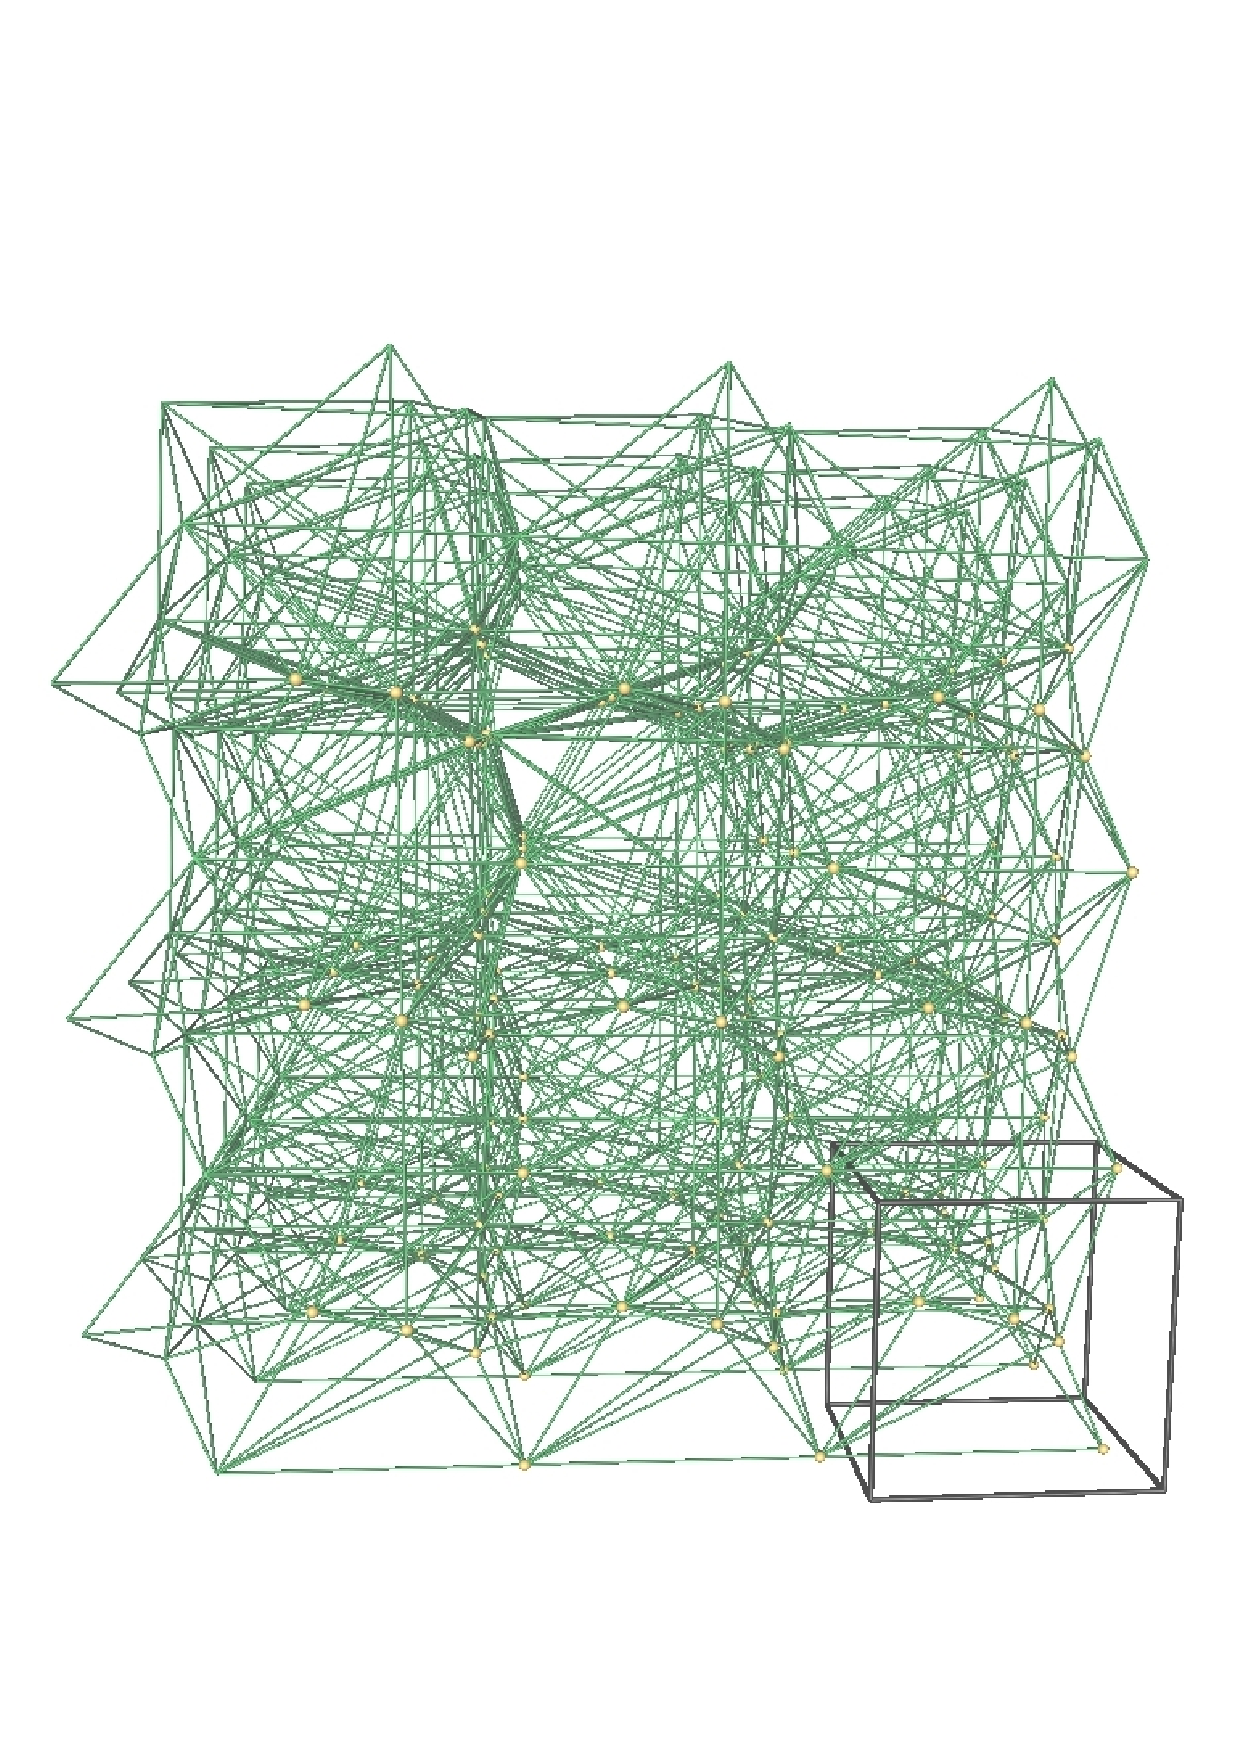
\includegraphics[width=5cm]{Periodic_3_triangulation_3_ref/it_STORED} 
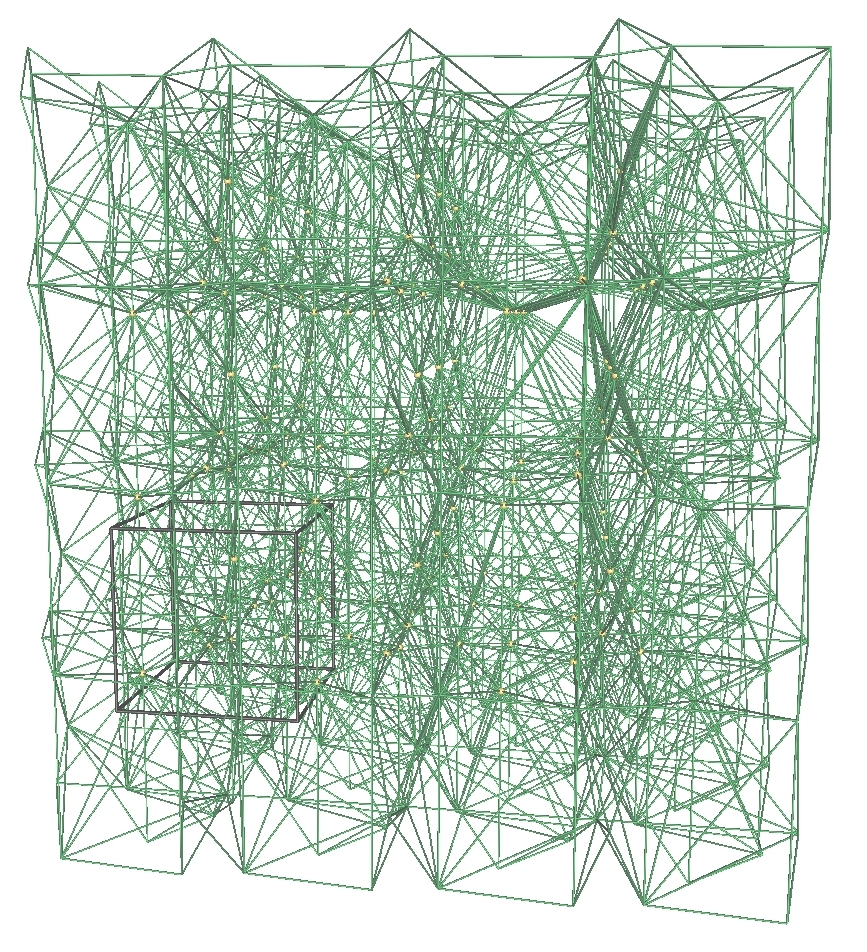
\includegraphics[width=5cm]{Periodic_3_triangulation_3_ref/it_STORED_COVER_DOMAIN}\\
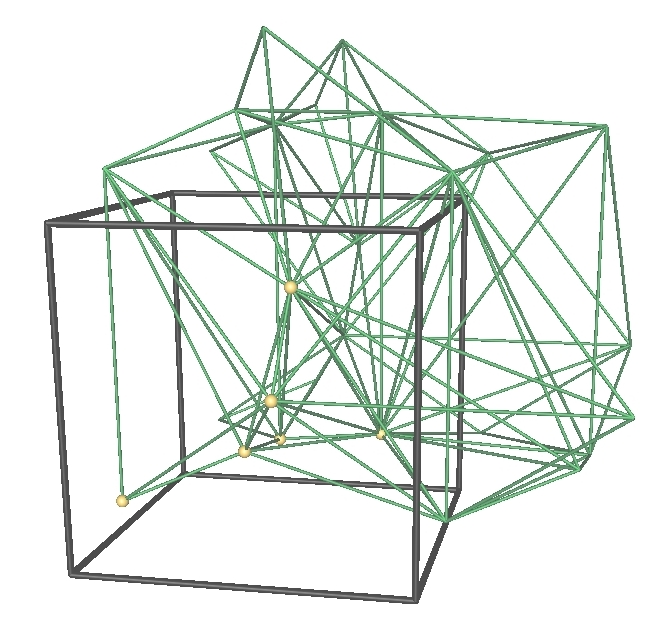
\includegraphics[width=5cm]{Periodic_3_triangulation_3_ref/it_UNIQUE} 
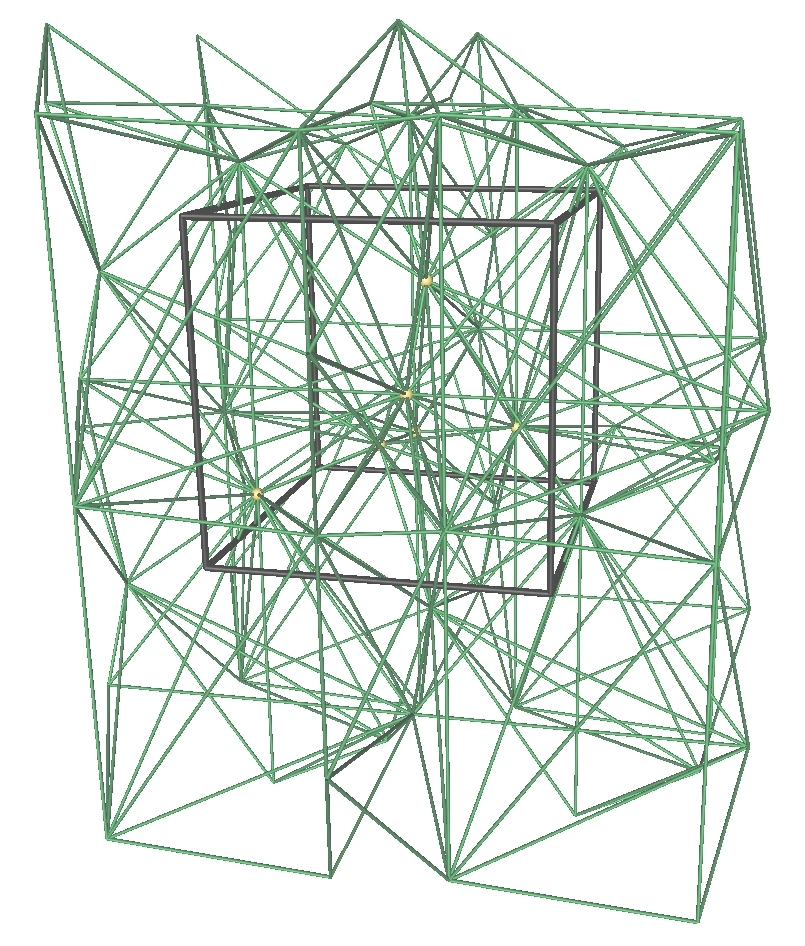
\includegraphics[width=5cm]{Periodic_3_triangulation_3_ref/it_UNIQUE_COVER_DOMAIN} 
\end{center}
\end{ccTexOnly}
\begin{ccHtmlOnly}
<CENTER>
<img border=0 src="./it_STORED_small.jpg" align=middle
  alt="STORED">
<img border=0 src="./it_STORED_COVER_DOMAIN_small.jpg" align=middle
  alt="STORED_COVER_DOMAIN">
<img border=0 src="./it_UNIQUE_small.jpg" align=middle
  alt="UNIQUE">
<img border=0 src="./it_UNIQUE_COVER_DOMAIN_small.jpg" align=middle
  alt="UNIQUE_COVER_DOMAIN">
</CENTER>
\end{ccHtmlOnly}
\caption{The four different modes of the geometric iterators: STORED,
  STORED\_COVER\_DOMAIN, UNIQUE, UNIQUE\_COVER\_DOMAIN. Note that in
  case of computing in 1-sheeted covering STORED and UNIQUE give the
  same result.
\label{P3Triangulation3-fig-geom_iterators}}
\end{figure} 


\ccThree{Periodic_tetrahedron_iterator}{XXXXXXX}{}

\ccMethod{Periodic_point_iterator periodic_points_begin(Iterator_type it =
  AS_STORED) const;}
{Iterates over the points of the triangulation. Its behavior is
  defined by the \ccc{Iterator_type} \ccc{it} as described on
  \ccRefPage{CGAL::Periodic_3_triangulation_3::Iterator_type}.}
\ccGlue
\ccMethod{Periodic_point_iterator periodic_points_end(Iterator_type it =
  AS_STORED) const;}
{Past-the-end iterator. Note that to match another
  \ccc{Periodic_point_iterator} both must have the same
  \ccc{Iterator_type} \ccc{it}.}

\ccMethod{Periodic_segment_iterator periodic_segments_begin(Iterator_type it =
  AS_STORED) const;}
{Iterates over the segments of the triangulation. Its behavior is
  defined by the \ccc{Iterator_type} \ccc{it} as described on
  \ccRefPage{CGAL::Periodic_3_triangulation_3::Iterator_type}.}
\ccGlue
\ccMethod{Periodic_segment_iterator periodic_segments_end(Iterator_type it =
  AS_STORED) const;}
{Past-the-end iterator. Note that to match another
  \ccc{Periodic_segment_iterator} both must have the same
  \ccc{Iterator_type} \ccc{it}.}

\ccMethod{Periodic_triangle_iterator periodic_triangles_begin(Iterator_type it =
  AS_STORED) const;}
{Iterates over the triangles of the triangulation. Its behavior is
  defined by the \ccc{Iterator_type} \ccc{it} as described on
  \ccRefPage{CGAL::Periodic_3_triangulation_3::Iterator_type}.}
\ccGlue
\ccMethod{Periodic_triangle_iterator periodic_triangles_end(Iterator_type it =
  AS_STORED) const;}
{Past-the-end iterator. Note that to match another
  \ccc{Periodic_triangle_iterator} both must have the same
  \ccc{Iterator_type} \ccc{it}.}

\ccMethod{Periodic_tetrahedron_iterator periodic_tetrahedra_begin(Iterator_type it =
  AS_STORED) const;} 
{Iterates over the tetrahedra of the triangulation. Its behavior is
  defined by the \ccc{Iterator_type} \ccc{it} as described on
  \ccRefPage{CGAL::Periodic_3_triangulation_3::Iterator_type}.}
\ccGlue
\ccMethod{Periodic_tetrahedron_iterator periodic_tetrahedra_end(Iterator_type it =
  AS_STORED) const;} 
{Past-the-end iterator. Note that to match another
  \ccc{Periodic_tetrahedron_iterator} both must have the same
  \ccc{Iterator_type} \ccc{it}.} 

\ccHeading{Cell and Facet Circulators}
\ccThree{Facet_circulator}{t.incident_facets(Edge e)xXXXXXXXXXXX}{}

The following circulators respectively visit all cells or all facets
incident to a given edge. They are non-mutable and bidirectional. They
are invalidated by any modification of one of the cells traversed. 

\ccMethod{Cell_circulator incident_cells(Edge e) const;}
{Starts at an arbitrary cell incident to \ccc{e}.}
\ccGlue
\ccMethod{Cell_circulator incident_cells(Cell_handle c, int i, int j) const;}
{As above for edge \ccc{(i,j)} of \ccc{c}.}
\ccGlue
\ccMethod{Cell_circulator incident_cells(Edge e, Cell_handle start) const;}
{Starts at cell \ccc{start}.
\ccPrecond{\ccc{start} is incident to \ccc{e}.}}
\ccGlue
\ccMethod{Cell_circulator incident_cells(Cell_handle c, int i, int j, 
Cell_handle start) const;}
{As above for edge \ccc{(i,j)} of \ccc{c}.}

\ccMethod{Facet_circulator incident_facets(Edge e) const;}
{Starts at an arbitrary facet incident to \ccc{e}.}
\ccGlue
\ccMethod{Facet_circulator incident_facets(Cell_handle c, int i, int j) const;}
{As above for edge \ccc{(i,j)} of \ccc{c}.} 
\ccGlue
\ccMethod{Facet_circulator incident_facets(Edge e, Facet start) const;}
{Starts at facet \ccc{start}. 
\ccPrecond{\ccc{start} is incident to \ccc{e}.}}
\ccGlue
\ccMethod{Facet_circulator incident_facets(Edge e, Cell_handle start, int f) 
const;}
{Starts at facet of index \ccc{f} in \ccc{start}.}
\ccGlue
\ccMethod{Facet_circulator incident_facets(Cell_handle c, int i, int j,
Facet start) const;} 
{As above for edge \ccc{(i,j)} of \ccc{c}.} 
\ccGlue
\ccMethod{Facet_circulator incident_facets(Cell_handle c, int i, int j,
Cell_handle start, int f) const;}
{As above for edge \ccc{(i,j)} of \ccc{c} and facet \ccc{(start,f)}.} 


\ccHeading{Traversal of the incident cells and facets, and the adjacent
vertices of a given vertex} 
\ccThree{OutputIterator}{t.inciden__cells()}{}

\ccMethod{template <class OutputIterator>
          OutputIterator
          incident_cells(Vertex_handle v, OutputIterator cells) const;}
{Copies the \ccc{Cell_handle}s of all cells incident to \ccc{v} to the output
iterator \ccc{cells}. Returns the resulting output iterator.
\ccPrecond{\ccc{v} $\neq$ \ccc{Vertex_handle()}, \ccVar.\ccc{is_vertex(v)}.}}

\ccMethod{template <class OutputIterator>
          OutputIterator
          incident_facets(Vertex_handle v, OutputIterator facets) const;}
{Copies the \ccc{Facet}s incident to \ccc{v} to the output iterator
\ccc{facets}.
Returns the resulting output iterator.
\ccPrecond{\ccc{v} $\neq$ \ccc{Vertex_handle()}, \ccVar.\ccc{is_vertex(v)}.}}

\ccMethod{template <class OutputIterator>
          OutputIterator
          incident_edges(Vertex_handle v, OutputIterator edges) const;}
{Copies the \ccc{Edge}s incident to \ccc{v} to the output iterator
\ccc{edges}.
Returns the resulting output iterator.
\ccPrecond{\ccc{v} $\neq$ \ccc{Vertex_handle()}, \ccVar.\ccc{is_vertex(v)}.}}

\ccMethod{template <class OutputIterator>
          OutputIterator
          adjacent_vertices(Vertex_handle v, OutputIterator vertices) const;}
{Copies the \ccc{Vertex_handle}s of all vertices adjacent to \ccc{v} to the
output iterator \ccc{vertices}.  Returns the resulting output iterator.
\ccPrecond{\ccc{v} $\neq$ \ccc{Vertex_handle()}, \ccVar.\ccc{is_vertex(v)}.}}

\ccMethod{size_type degree(Vertex_handle v) const;}
{Returns the degree of a vertex, that is, the number of adjacent vertices.
\ccPrecond{\ccc{v} $\neq$ \ccc{Vertex_handle()}, \ccVar.\ccc{is_vertex(v)}.}}

\ccHeading{Traversal between adjacent cells}
\ccThree{Vertex_handle}{mirror_vertex( Cell_handle c, int i)X}{}

\ccMethod{int mirror_index(Cell_handle c, int i) const;}
{Returns the index of \ccc{c} in its $i^{th}$ neighbor.
\ccPrecond{$i \in \{0, 1, 2, 3\}$.}}
\ccGlue
\ccMethod{Vertex_handle mirror_vertex(Cell_handle c, int i) const;}
{Returns the vertex of the $i^{th}$ neighbor of \ccc{c} that is opposite to
\ccc{c}.
\ccPrecond{$i \in \{0, 1, 2, 3\}$.}}
\ccGlue
\ccMethod{Facet mirror_facet(Facet f) const;}
{Returns the same facet viewed from the other adjacent cell.}

\begin{ccAdvanced}
\ccHeading{Checking}
\ccThree{ostream&}{XXXXXXXX}{}

The responsibility of keeping a valid triangulation belongs to the user
when using advanced operations allowing a direct manipulation of cells
and vertices. We provide the user with the following methods to help
debugging. 

\ccMethod{bool
          is_valid(bool verbose = false) const;}
{Checks the combinatorial validity of the triangulation. Checks also the
validity of its geometric embedding (see
Section~\ref{P3Triangulation3-sec-intro}).\\ When \ccc{verbose}
is set to true, messages describing the first invalidity encountered
are printed.} 

\ccMethod{bool
          is_valid(Cell_handle c, bool verbose = false) const;}
{Checks the combinatorial validity of the cell by calling the
\ccc{is_valid} method of the \ccc{Triangulation_data_structure} cell
class. Also checks the geometric validity of \ccc{c}, if \ccc{c} is
finite. (See Section~\ref{P3Triangulation3-sec-intro}.)\\ 
When \ccc{verbose} is set to \ccc{true}, messages are printed to give
a precise indication of the kind of invalidity encountered.}

\end{ccAdvanced}

\ccHeading{I/O}
\ccThree{ostream&}{ostream& os XX Periodic_3_triangulation_3 tX}{}

\ccFunction{istream& operator>> (istream& is, Periodic_3_triangulation_3 &t);}
{Reads a triangulation from \ccc{is} and stores it in \ccc{t}.
\ccPrecond{\ccc{is} has the below described format.}}

\ccFunction{ostream& operator<< (ostream& os, const Periodic_3_triangulation_3 &t);}
{Writes the triangulation \ccc{t} into \ccc{os}.}

The information in the \ccc{iostream} is:
\begin{itemize}
\item the original domain
\item the number of sheets of the covering as in
  \ccc{number_of_sheets()}
\item the number of vertices
\item the non-combinatorial information of vertices (point
  resp. point-offset pairs, etc.)
\item the number of cells
\item the indices of the vertices of each cell
\item the indices of the neighbors of each cell, where the index
  corresponds to the preceding list of cells
\item the offsets corresponding to the vertices of the cells
\item the non-combinatorial information of each cell
\end{itemize}

\ccSeeAlso

\ccc{Periodic_3_Delaunay_triangulation_3}

%\ccExample
%%\ccIncludeExampleCode{Triangulation3/example1.cpp}

\end{ccRefClass}
